\documentclass[preprint,12pt]{elsarticle}
\journal{Computers in Biology and Medicine}
\usepackage[margin=1in]{geometry}
\usepackage[T1]{fontenc}
\usepackage{amsmath,amsfonts,amssymb}
\usepackage{booktabs}
\usepackage{multirow}
\usepackage{graphicx}
\usepackage{xcolor}
\usepackage{bm}
\usepackage{array}
\usepackage{lineno}
\usepackage{setspace}
\usepackage{tikz}
\usetikzlibrary{shapes.geometric, arrows.meta, positioning, fit, backgrounds, calc, shadows}
\usepackage{url}
\usepackage{hyperref}
\hypersetup{colorlinks=true,linkcolor=blue,citecolor=blue,urlcolor=blue}
\biboptions{numbers,sort&compress}
\begin{document}
\linenumbers
\modulolinenumbers[1]
\doublespacing
\begin{frontmatter}
\title{VERA-ECG: Verifiable Evidential Reasoning and Anatomy-Grounded Multimodal Framework for Reliable 12-Lead ECG Interpretation}
\author[1]{Yihao Wen}
\author[2]{Jun Zeng}
\affiliation[1]{organization={Taiyuan University of Technology}, city={Taiyuan}, postcode={030024}, country={China}}
\affiliation[2]{organization={Chongqing University of Posts and Telecommunications}, city={Chongqing}, postcode={400065}, country={China}}
\cortext[cor1]{Corresponding author.}
\ead[cor1]{wenyihao239@gmail.com}
\ead{zeng.cqupt@gmail.com}
\begin{abstract}
Multimodal large language models (MLLMs) combining ECG time series, waveform images, and text are promising but face modality polarization, non-random interval missingness, loss of millivolt scale, and unreliable clinical grounding. We propose VERA-ECG, a verifiable evidential and anatomy-grounded framework. Multi-label Beta-evidential fusion (TMC/PC-BEF) models class-wise positive/negative evidence and epistemic uncertainty with hardware-quality discounting. An anatomy-grouped presence-gated evidence bottleneck (APEB) converts missing intervals into presence-gated features and enforces a one-way differentiable clinical logic loss (A8-OneWay) across four coronary territories. Class-balanced feature calibration addresses cross-center prior shift. Soft multimodal tokens, including longitudinal differential tokens, are combined with hard symbolic anchors in a 3B MLLM (HE-DVR). On PTB-XL, CPSC2018, and ECG-QA, VERA-ECG achieves 0.9205 $\pm$ 0.0006 macro-AUROC and 0.68\% diagnostic--evidence contradiction (A7: 0.88\%), with a counterfactual sensitivity ratio of 7.12 ($\Delta$logit ratio 8.70). C0 reaches 0.9104 five-fold mean CPSC2018 macro-AUROC, improving same-fold Fold0 from 0.8603 to 0.9080 and ST-elevation AUROC from 0.670 to 0.8123. HE-DVR reaches 63.63\% legacy and 59.83\% set exact match on 6,330 ECG-QA questions.
\end{abstract}
\begin{keyword}
Electrocardiogram (ECG), Multimodal Large Language Models, Evidential Deep Learning, Neuro-Symbolic Reasoning, Cross-Domain Generalization.
\end{keyword}
\end{frontmatter}
\maketitle


\section{Introduction}
The standard 12-lead electrocardiogram (ECG) is the cornerstone of non-invasive cardiovascular diagnostics, naturally encompassing three complementary modalities: 1D high-resolution physiological time-series signals ($12 \times T$), 2D spatially formatted waveform images ($H \times W \times 3$), and structured clinical reports or diagnostic queries. Unlike memory-prohibitive 3D radiological volumes (CT/MRI) or gigapixel whole-slide pathology images (WSI), 12-lead ECGs allow lightweight modality encoders to be paired with large language models (LLMs) on consumer-grade hardware. Recently, ECG multimodal large language models (ECG MLLMs)---such as GEM \cite{gem2025}, PULSE \cite{pulse2026}, HeartcareGPT \cite{heartcare2026}, and ECG-R1 \cite{ecgr1_2026}---have progressed from single-modality alignment to dual-modality encoding (1D signal + 2D image) and protocol-guided chain-of-thought (CoT) reasoning.

Despite these advances, deploying ECG multimodal models in realistic clinical workflows reveals four fundamental vulnerabilities that remain unresolved by existing concatenation or modality-dropout architectures:

\begin{enumerate}
    \item \textbf{Silent Failure of Naive Quality Gating and Modality Polarization:} In clinical practice, modalities rarely vanish completely; instead, they undergo continuous, asymmetric degradation (e.g., baseline wander, electrode drop, or blurred/cropped paper scans). Our motivating empirical audit reveals that when explicit signal/image quality metrics ($\bm{q}_s, \bm{q}_i$) are concatenated with high-dimensional latent features into a multilayer perceptron (MLP) gate, permuting $\bm{q}$ across test samples yields virtually zero performance change ($\Delta\text{AUC} \approx 10^{-5}$). Worse, due to the natural performance gap between 1D signal encoders and 2D image encoders, standard gates polarize to extreme binary weights ($\alpha_s \to 0.00001$ or $0.9998$), discarding valuable complementary evidence under mild corruption.
    \item \textbf{Informative Missingness and Scalar Bottleneck Collapse:} Enforcing clinical evidence grounding requires predicting physiological intervals (HR, PR, QRS, QT, QTc) and lead-level abnormalities. However, rule-based waveform delineators (e.g., NeuroKit2) fail to extract valid PR intervals on \textbf{41.5\%} of clinical test recordings---primarily because atrial fibrillation (AF) physiologically abolishes sinus P-waves. Forcing a continuous scalar bottleneck over globally pooled 100 Hz features collapses PR and QRS Pearson correlations to $0.180$ and $0.145$, respectively, while lacking spatial coronary territory grounding.
    \item \textbf{In-Domain vs. Cross-Domain Tension in Millivolt ($\text{mV}$) Scaling:} Standard deep learning pipelines apply per-sample, per-lead z-score normalization, which stabilizes rhythm recognition (e.g., AF, bundle branch blocks) but erases absolute millivolt thresholds required for diagnosing ST-segment elevation (STE, $\ge 0.1\text{--}0.2\text{ mV}$) and depression (STD). Conversely, naively injecting raw amplitude statistics via Feature-wise Linear Modulation (FiLM) boosts in-domain accuracy but suffers from out-of-distribution (OOD) gain shifts and severe source-domain long-tail bias (e.g., only 27 STE cases in PTB-XL) when transferred zero-shot across hospitals.
    \item \textbf{Diagnostic-Evidence Contradictions and Longitudinal Reasoning Gaps:} MLLMs projecting continuous ECG embeddings into soft tokens still exhibit up to $15\%$ interval estimation error \cite{ecgr1_2026} and frequently predict high-level diagnoses that contradict their own intermediate evidence predictions. Furthermore, existing MLLMs struggle with longitudinal comparison queries (\texttt{Comparison-Consecutive} in ECG-QA \cite{ecgqa2023}) that require identifying newly emerged or resolved symptoms across serial ECGs.
\end{enumerate}

To overcome these challenges, we propose \textbf{VERA-ECG} (\emph{Verifiable Evidential Reasoning and Anatomy-Grounded Multimodal Framework}). Rather than treating multimodal fusion and clinical reasoning as black-box feature concatenation, VERA-ECG establishes a verifiable pipeline spanning physical scale preservation, Subjective Logic evidential fusion, neuro-symbolic anatomical bottlenecks, and hybrid soft-hard LLM prompting. Our primary contributions are summarized as follows:

\begin{itemize}
    \item \textbf{Empirical Discovery and Multi-Label Beta-Evidential Fusion (TMC / PC-BEF):} We systematically expose the gate polarization and permutation insensitivity of conventional quality-gated fusion. We formulate a multi-label Beta-evidential fusion framework that models class-wise positive/negative belief masses and epistemic uncertainty, achieving \textbf{0.9201 $\pm$ 0.0008} clean AUROC, \textbf{0.9009 $\pm$ 0.0005} dual-corruption AUROC, and a $53\%$ reduction in Expected Calibration Error (ECE \textbf{0.0125}), alongside a prior-discounted variant (\textbf{PC-BEF}) that restores explicit quality controllability ($\Delta\text{AUC}_{\text{perm}} = 0.01574$).
    \item \textbf{Anatomy-Grouped Presence-Gated Evidence Bottleneck (APEB):} We transform non-random interval missingness into a diagnostic validity gate (AUC \textbf{0.8570}) combined with clinical ordinal bucketing and four coronary anatomical territories (Inferior, Septal, Anterior, Lateral). By introducing a \textbf{one-way differentiable clinical logic loss} (\textbf{A8-OneWay}) that detaches diagnostic gradients during evidence alignment, we achieve the highest diagnostic AUROC in our study (\textbf{0.9205 $\pm$ 0.0006}), reduce diagnostic--evidence contradiction from $0.88\%$ (A7) to \textbf{0.68\%} with A8-OneWay, and achieve a counterfactual lead-masking sensitivity ratio (CSR) of \textbf{7.12} ($\Delta\text{logit}$ ratio \textbf{8.70}).
    \item \textbf{Millivolt-Preserving Encoding and Cross-Center Calibration:} We demonstrate that FiLM-based millivolt injection (\textbf{A0-mV}) elevates in-domain PTB-XL AUROC from $0.8988$ to \textbf{0.9189} ($5$-class) and \textbf{0.9224} ($9$-class). For cross-center transfer to CPSC2018 ($5$-fold evaluation), we uncover the coupling between OOD amplitude drift and source long-tail bias, showing that class-balanced linear probing restores A0-mV from $0.8192$ to \textbf{0.9024}, while balanced morphological representations (\textbf{C0}) reach \textbf{0.9104} (raising STE AUROC from $0.670$ to \textbf{0.8123}).
    \item \textbf{Hybrid Evidence Injection for 3B MLLM Reasoning (HE-DVR):} On a single consumer GPU (16GB VRAM), we integrate 24 multimodal soft tokens ($\langle\text{ECG\_A}\rangle$, $\langle\text{ECG\_B}\rangle$, and differential tokens $\langle\text{ECG\_D}\rangle$) with explicit APEB symbolic anchors into Qwen2.5-3B-Instruct, achieving \textbf{63.63\%} legacy Exact Match (\textbf{59.83\%} strict Set EM, \textbf{61.99\%} Set F1) across all 6,330 test samples in ECG-QA.
\end{itemize}

\section{Related Work}
\subsection{Multimodal ECG Representation and MLLMs}
Early self-supervised ECG models focused on 1D signal pretraining (e.g., ECG-FM, C-MELT, ECG-CoCa) or 2D waveform image adaptation. Recently, PULSE \cite{pulse2026} synthesized 1M+ realistic ECG images (\texttt{ECGInstruct}) to train vision-language models, but purely visual encoding loses millisecond-level interval precision. GEM \cite{gem2025} unified 1D time series, 2D images, and text via dual encoders and \texttt{FeatureDB}-assisted GPT-4o grounding (\texttt{ECG-Grounding-30k}). ECG-R1 \cite{ecgr1_2026} further introduced interleaved modality dropout (IMD) and reinforcement learning with diagnostic evidence rewards (EDER). However, OpenReview audits of ECG-R1 revealed that LLM-generated interval measurements still suffer from $15.16\%\text{--}15.34\%$ relative errors and underperform on rare critical abnormalities due to top-frequency sampling bias \cite{ecgr1_2026}. ECG-MTDA \cite{ecgmtda2026} decoupled morphology and rhythm for text alignment, while MEETI \cite{meeti2026} expanded MIMIC-IV-ECG with LLM interpretations. Unlike prior works that rely on static concatenation or heuristic dropout, VERA-ECG introduces Subjective Logic uncertainty quantification and neuro-symbolic anatomical consistency.

\subsection{Evidential Deep Learning and Neuro-Symbolic Bottlenecks}
Trusted Multi-View Classification (TMC) \cite{tmc2023} and recent extensions (CCML \cite{ccml2025}, TMUR \cite{tmur2026}) model view-specific uncertainty via Dirichlet distributions. However, Dirichlet parameterizations assume mutually exclusive single-label classes ($\sum_k p_k = 1$), violating the multi-label comorbidity structure of clinical ECGs. Furthermore, Concept Bottleneck Models (CBMs) assume fully observed intermediate concepts, breaking down when physiological features (such as P-waves in atrial fibrillation) are pathologically absent. Our APEB module bridges this gap via presence-gated interval bottlenecks and one-way \L{}ukasiewicz logic regularization.

\section{Methodology: The VERA-ECG Framework}

\begin{figure}[htbp]
\centering
\resizebox{0.99\linewidth}{!}{%
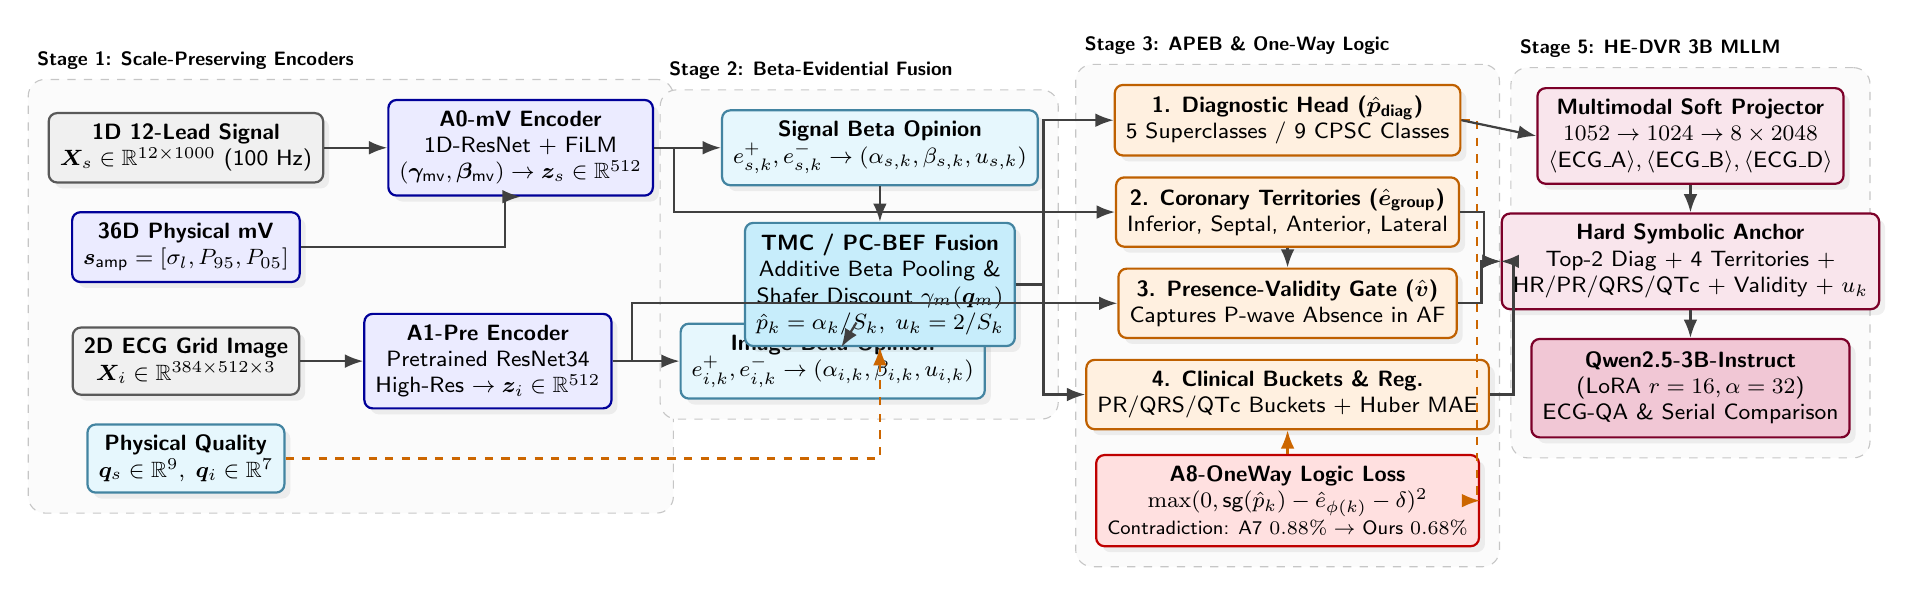
\begin{tikzpicture}[
    font=\sffamily\footnotesize,
    >=Latex,
    node distance=0.45cm and 0.65cm,
    box/.style={draw=black!75, rounded corners=3pt, thick, align=center, minimum height=0.85cm, inner sep=4pt, drop shadow={opacity=0.12}},
    stage1/.style={box, fill=blue!8, draw=blue!60!black},
    stage2/.style={box, fill=cyan!10, draw=cyan!60!black},
    stage3/.style={box, fill=orange!12, draw=orange!75!black},
    stage5/.style={box, fill=purple!10, draw=purple!65!black},
    inputbox/.style={box, fill=gray!12, draw=gray!70!black, minimum width=2.4cm},
    stagebg/.style={draw=gray!45, dashed, rounded corners=6pt, inner sep=7pt, fill=gray!3},
    arrow/.style={->, thick, draw=black!75},
    darrow/.style={->, thick, dashed, draw=orange!80!black}
]

% ==================== STAGE 1: Inputs & Encoders ====================
\node[inputbox] (sig_in) {\textbf{1D 12-Lead Signal}\\$\bm{X}_s \in \mathbb{R}^{12 \times 1000}$ (100 Hz)};
\node[stage1, below=0.35cm of sig_in, minimum width=2.4cm] (mv_stat) {\textbf{36D Physical mV}\\$\bm{s}_{\text{amp}} = [\sigma_l, P_{95}, P_{05}]$};
\node[inputbox, below=0.55cm of mv_stat] (img_in) {\textbf{2D ECG Grid Image}\\$\bm{X}_i \in \mathbb{R}^{384 \times 512 \times 3}$};
\node[stage2, below=0.35cm of img_in, minimum width=2.4cm] (qual_in) {\textbf{Physical Quality}\\$\bm{q}_s \in \mathbb{R}^9, \; \bm{q}_i \in \mathbb{R}^7$};

\node[stage1, right=0.8cm of sig_in, minimum width=2.7cm, minimum height=1.2cm] (enc_s) {\textbf{A0-mV Encoder}\\1D-ResNet + FiLM\\$(\bm{\gamma}_{\text{mv}}, \bm{\beta}_{\text{mv}}) \to \bm{z}_s \in \mathbb{R}^{512}$};
\node[stage1, right=0.8cm of img_in, minimum width=2.7cm, minimum height=1.2cm] (enc_i) {\textbf{A1-Pre Encoder}\\Pretrained ResNet34\\High-Res $\to \bm{z}_i \in \mathbb{R}^{512}$};

\draw[arrow] (sig_in) -- (enc_s);
\draw[arrow] (mv_stat.east) -| ([xshift=-0.2cm]enc_s.south) -- (enc_s.south);
\draw[arrow] (img_in) -- (enc_i);

% ==================== STAGE 2: Evidential Fusion ====================
\node[stage2, right=0.85cm of enc_s, minimum width=3.1cm] (evid_s) {\textbf{Signal Beta Opinion}\\$e_{s,k}^+, e_{s,k}^- \to (\alpha_{s,k}, \beta_{s,k}, u_{s,k})$};
\node[stage2, right=0.85cm of enc_i, minimum width=3.1cm] (evid_i) {\textbf{Image Beta Opinion}\\$e_{i,k}^+, e_{i,k}^- \to (\alpha_{i,k}, \beta_{i,k}, u_{i,k})$};
\node[stage2, below=0.45cm of evid_s, minimum width=3.1cm, fill=cyan!22] (tmc_fuse) {\textbf{TMC / PC-BEF Fusion}\\Additive Beta Pooling \&\\Shafer Discount $\gamma_m(\bm{q}_m)$\\$\hat{p}_k = \alpha_k / S_k, \; u_k = 2/S_k$};

\draw[arrow] (enc_s) -- (evid_s);
\draw[arrow] (enc_i) -- (evid_i);
\draw[arrow] (evid_s) -- (tmc_fuse);
\draw[arrow] (evid_i) -- (tmc_fuse);
\draw[darrow] (qual_in.east) -| (tmc_fuse.south);

% ==================== STAGE 3: APEB Neuro-Symbolic Bottleneck ====================
\node[stage3, right=0.95cm of evid_s, yshift=0.35cm, minimum width=3.3cm] (head_diag) {\textbf{1. Diagnostic Head ($\hat{\bm{p}}_{\text{diag}}$)}\\5 Superclasses / 9 CPSC Classes};
\node[stage3, below=0.25cm of head_diag, minimum width=3.3cm] (head_group) {\textbf{2. Coronary Territories ($\hat{\bm{e}}_{\text{group}}$)}\\Inferior, Septal, Anterior, Lateral};
\node[stage3, below=0.25cm of head_group, minimum width=3.3cm] (head_valid) {\textbf{3. Presence-Validity Gate ($\hat{\bm{v}}$)}\\Captures P-wave Absence in AF};
\node[stage3, below=0.25cm of head_valid, minimum width=3.3cm] (head_bucket) {\textbf{4. Clinical Buckets \& Reg.}\\PR/QRS/QTc Buckets + Huber MAE};

\node[box, fill=red!12, draw=red!75!black, below=0.3cm of head_bucket, minimum width=3.3cm] (logic_loss) {\textbf{A8-OneWay Logic Loss}\\$\max(0, \text{sg}(\hat{p}_k) - \hat{e}_{\phi(k)} - \delta)^2$\\{\scriptsize Contradiction: A7 $0.88\% \to$ Ours $0.68\%$}};

\coordinate (z_concat) at ($(evid_s.east)!0.5!(evid_i.east) + (0.42cm, 0)$);
\draw[arrow] (enc_s.east) -- ++(0.25,0) |- (head_group.west);
\draw[arrow] (enc_i.east) -- ++(0.25,0) |- (head_valid.west);
\draw[arrow] (tmc_fuse.east) -- ++(0.35,0) |- (head_diag.west);
\draw[arrow] (tmc_fuse.east) -- ++(0.35,0) |- (head_bucket.west);
\draw[darrow] (head_diag.east) -- ++(0.2,0) |- (logic_loss.east);
\draw[arrow] (head_group.south) -- (head_valid.north);
\draw[darrow] (logic_loss.north) -- (head_bucket.south);

% ==================== STAGE 5: HE-DVR MLLM ====================
\node[stage5, right=0.95cm of head_diag, yshift=-0.2cm, minimum width=3.3cm] (soft_proj) {\textbf{Multimodal Soft Projector}\\$1052 \to 1024 \to 8 \times 2048$\\$\langle\text{ECG\_A}\rangle, \langle\text{ECG\_B}\rangle, \langle\text{ECG\_D}\rangle$};
\node[stage5, below=0.35cm of soft_proj, minimum width=3.3cm] (hard_anchor) {\textbf{Hard Symbolic Anchor}\\Top-2 Diag + 4 Territories +\\HR/PR/QRS/QTc + Validity + $u_k$};
\node[stage5, below=0.35cm of hard_anchor, minimum width=3.3cm, minimum height=1.25cm, fill=purple!22] (qwen_llm) {\textbf{Qwen2.5-3B-Instruct}\\(LoRA $r=16, \alpha=32$)\\ECG-QA \& Serial Comparison};

\draw[arrow] (head_diag.east) -- (soft_proj.west);
\draw[arrow] (head_group.east) -- ++(0.3,0) |- (hard_anchor.west);
\draw[arrow] (head_valid.east) -- ++(0.3,0) |- (hard_anchor.west);
\draw[arrow] (head_bucket.east) -- ++(0.3,0) |- (hard_anchor.west);
\draw[arrow] (soft_proj) -- (hard_anchor);
\draw[arrow] (hard_anchor) -- (qwen_llm);

% Background Stage Boxes
\begin{scope}[on background layer]
    \node[stagebg, fit=(sig_in)(qual_in)(enc_s)(enc_i), label={[font=\sffamily\bfseries\scriptsize, anchor=south west]north west:Stage 1: Scale-Preserving Encoders}] {};
    \node[stagebg, fit=(evid_s)(evid_i)(tmc_fuse), label={[font=\sffamily\bfseries\scriptsize, anchor=south west]north west:Stage 2: Beta-Evidential Fusion}] {};
    \node[stagebg, fit=(head_diag)(logic_loss), label={[font=\sffamily\bfseries\scriptsize, anchor=south west]north west:Stage 3: APEB \& One-Way Logic}] {};
    \node[stagebg, fit=(soft_proj)(qwen_llm), label={[font=\sffamily\bfseries\scriptsize, anchor=south west]north west:Stage 5: HE-DVR 3B MLLM}] {};
\end{scope}

\end{tikzpicture}%
}
\caption{Overview of the \textbf{VERA-ECG} framework. \textbf{Stage 1} preserves physical millivolt (mV) scales via 36D FiLM modulation (\textbf{A0-mV}) paired with high-resolution visual encoding (\textbf{A1-Pre}). \textbf{Stage 2} models positive/negative Beta beliefs and epistemic uncertainty (\textbf{TMC / PC-BEF}). \textbf{Stage 3} grounds predictions into 4 coronary territories, interval validity gates, and clinical buckets via a one-way differentiable logic loss (\textbf{A8-OneWay}) that detaches diagnostic gradients ($\text{sg}(\hat{p}_k)$). \textbf{Stage 5} injects soft tokens ($\langle\text{ECG\_A/B/D}\rangle$) and hard APEB symbolic anchors into Qwen2.5-3B-Instruct.}
\label{fig:architecture}
\end{figure}

\subsection{Motivating Empirical Audit: Why Naive Gating and Scalar Bottlenecks Fail}
Before introducing VERA-ECG, we conduct a rigorous empirical audit of conventional multimodal fusion and evidence bottlenecks on PTB-XL ($n=21,388$):
\begin{enumerate}
    \item \textbf{Permutation Insensitivity of Concatenated Quality Gates:} In a baseline quality-aware gate (\textbf{A6}), 9 signal quality features $\bm{q}_s \in \mathbb{R}^9$ (SNR, baseline ratio, high-frequency ratio, missing/flat/clip ratio, lead correlation, kurtosis, amplitude) and 7 image quality features $\bm{q}_i \in \mathbb{R}^7$ (Laplacian variance, contrast, brightness, margin ratios, edge density) are concatenated with latent features $[\bm{z}_s; \bm{z}_i] \in \mathbb{R}^{1024}$ to predict gating weights $[\alpha_s, \alpha_i]$. Randomly permuting $\bm{q}$ across test samples 10 times produces $\Delta\text{AUC} = 0.00001$ on clean data and $-0.00018\text{ to }0.00001$ across 6 corrupted conditions, indicating that high-dimensional latent norms can dominate explicit low-dimensional quality inputs.
    \item \textbf{Gate Polarization:} Because scratch-trained 2D image encoders ($0.8556$ AUC) lag behind 1D signal encoders ($0.8991$ AUC), \textbf{A6} collapses to binary extremes: under 10 dB signal noise, $\alpha_s$ drops to $0.00001$ (discarding a signal that still achieves $0.878$ AUC alone), whereas under image blur/JPEG compression, $\alpha_s$ saturates at $0.9991\text{--}0.9998$, underperforming a constant $0.5$ gate ($0.9017$ vs. $0.9077$).
    \item \textbf{PR Missingness and Scalar Bottleneck Degradation:} Delineating 500 Hz signals via NeuroKit2 yields $99.9\%$ coverage on HR but only \textbf{58.5\%} test coverage on PR intervals due to P-wave absence in arrhythmias. Enforcing a strict 5-scalar bottleneck (\textbf{B4'}) degrades PR and QRS correlations from $0.485/0.524$ (\textbf{B1}) down to $0.180/0.145$.
\end{enumerate}

\subsection{Stage 1: Millivolt-Preserving Signal Encoding (A0-mV) and High-Resolution Visual Encoding (A1-Pre)}
Let $\bm{X}_s \in \mathbb{R}^{12 \times T}$ ($T=1000$ at $100\text{ Hz}$) denote the raw 12-lead ECG signal in physical millivolts ($\text{mV}$), and $\bm{X}_i \in \mathbb{R}^{3 \times H \times W}$ denote the rendered 12-lead waveform image ($4 \times 3$ clinical layout plus a lead II rhythm strip on standard millimeter grid).

To prevent per-lead z-score normalization $\tilde{x}_{l,t} = (x_{l,t} - \mu_l)/\sigma_l$ from erasing physical ST-segment voltage elevations, \textbf{A0-mV} extracts a 36-dimensional physical amplitude descriptor prior to normalization:
\begin{equation}
    \bm{s}_{\text{amp}} = \bigoplus_{l=1}^{12} \left[ \sigma_l, \, P_{95}(\bm{x}_l), \, P_{05}(\bm{x}_l) \right] \in \mathbb{R}^{36},
\end{equation}
where $\sigma_l$, $P_{95}$, and $P_{05}$ represent the physical standard deviation, 95th percentile peak voltage, and 5th percentile trough voltage (in $\text{mV}$) of lead $l$. These descriptors capture a global voltage scale, not a local J-point ST offset: they restore the absolute energy removed by per-lead z-scoring, while the ST decision still comes from the learned waveform representation. While $\tilde{\bm{X}}_s$ is processed by a 4-stage 1D-ResNet ($C \in \{64, 128, 256, 512\}$), $\bm{s}_{\text{amp}}$ is projected through a lightweight MLP to generate Feature-wise Linear Modulation (FiLM) parameters $(\bm{\gamma}_{\text{mv}}, \bm{\beta}_{\text{mv}})$ injected into the high-level representation:
\begin{equation}
    \bm{z}_s = \text{GAP}\Big( (1 + \bm{\gamma}_{\text{mv}}(\bm{s}_{\text{amp}})) \odot \mathcal{F}_{\text{1D}}(\tilde{\bm{X}}_s) + \bm{\beta}_{\text{mv}}(\bm{s}_{\text{amp}}) \Big) \in \mathbb{R}^{512}.
\end{equation}
For the visual branch (\textbf{A1-Pre}), instead of downsampling images to $224 \times 224$ from scratch, we preserve a $384 \times 512$ resolution using an ImageNet-pretrained ResNet34 backbone to resolve millimeter-grid deflections ($\bm{z}_i \in \mathbb{R}^{512}$).

\subsection{Stage 2: Multi-Label Beta-Evidential Fusion (TMC \& PC-BEF)}
Because clinical ECGs exhibit multi-label comorbidities, we replace single-label Dirichlet distributions with $K$ independent Binomial/Beta subjective opinions $\omega_{m,k} = (b_{m,k}^+, b_{m,k}^-, u_{m,k})$ for each modality $m \in \{s, i\}$ and diagnostic class $k \in \{1, \dots, K\}$. Each modality head outputs non-negative positive evidence (supporting disease presence) and negative evidence (supporting absence) via Softplus activation:
\begin{equation}
\begin{aligned}
    e_{m,k}^+ &= \text{Softplus}(f_{m,k}^+(\bm{z}_m)) + 10^{-6},\\
    e_{m,k}^- &= \text{Softplus}(f_{m,k}^-(\bm{z}_m)) + 10^{-6}.
\end{aligned}
\end{equation}

We investigate two complementary evidential fusion paradigms:
\subsubsection{Unbiased Multi-Label Evidential Accumulation (TMC)}
In our primary accuracy-optimal formulation (\textbf{TMC}), evidence from both modalities is additively pooled per class: $e_{f,k}^+ = e_{s,k}^+ + e_{i,k}^+$ and $e_{f,k}^- = e_{s,k}^- + e_{i,k}^-$, yielding Beta distribution parameters $\alpha_k = e_{f,k}^+ + 1$, $\beta_k = e_{f,k}^- + 1$, total evidential strength $S_k = \alpha_k + \beta_k$, expected probability $\hat{p}_k = \alpha_k / S_k$, and epistemic uncertainty $u_k = 2 / S_k$. Here $e^\pm$ are learned class-wise evidence, not direct probability labels; $\hat p_k$ is the expected probability and $u_k$ is an epistemic mass. We therefore evaluate calibration, uncertainty discrimination, and corruption behavior separately rather than treating them as interchangeable.

\subsubsection{Prior-Discounted Conflict-Aware Evidential Fusion (PC-BEF)}
To enforce explicit hardware quality sensitivity, \textbf{PC-BEF} avoids concatenating $\bm{q}_m$ with $\bm{z}_m$. Instead, $\bm{q}_m$ parameterizes a Shafer reliability discounting factor $\gamma_m(\bm{q}_m) = \sigma(\text{MLP}_m(\bm{q}_m))$ that directly scales modality evidence: $\tilde{e}_{m,k}^\pm = \gamma_m(\bm{q}_m) e_{m,k}^\pm$. With belief masses $b_{m,k}^\pm = \tilde{e}_{m,k}^\pm / S_{m,k}$ and uncertainty $u_{m,k} = 2 / S_{m,k}$, cross-modal conflict is measured as $C_k = b_{s,k}^+ b_{i,k}^- + b_{s,k}^- b_{i,k}^+$, and beliefs are combined via Dempster-Shafer orthogonal summation:
\begin{equation}
    b_{f,k}^+ = \frac{b_{s,k}^+ b_{i,k}^+ + b_{s,k}^+ u_{i,k} + b_{i,k}^+ u_{s,k}}{1 - C_k}, \quad u_{f,k} = \frac{u_{s,k} u_{i,k}}{1 - C_k}.
\end{equation}
In \textbf{PC-BEF-v2}, we bound $\gamma_s \in [0.70, 1.0]$ and $\gamma_i \in [0.45, 1.0]$ and blend $0.5\text{ TMC} + 0.5\text{ PC-BEF}$ to study the Pareto trade-off between clean accuracy and explicit $\bm{q}$-permutation sensitivity. Models are trained with Bayes risk Digamma cross-entropy and annealed KL divergence.

\subsection{Stage 3: Anatomy-Grouped Presence-Gated Evidence Bottleneck (APEB) and One-Way Logic Consistency}
Given the concatenated multimodal representation $\bm{z} = [\bm{z}_s; \bm{z}_i] \in \mathbb{R}^{1024}$, \textbf{APEB} projects $\bm{z}$ through a shared 2-layer MLP trunk into five structured neuro-symbolic heads:
\begin{enumerate}
    \item \textbf{Diagnostic Head ($\hat{\bm{p}}_{\text{diag}} \in [0,1]^5$):} Predicts 5 superclass probabilities (\texttt{NORM, MI, STTC, CD, HYP}).
    \item \textbf{Coronary Anatomical Territory Head ($\hat{\bm{e}}_{\text{group}} \in [0,1]^4$):} Grounds spatial abnormalities into four standard anatomical lead groups derived from PTB-XL SCP codes and ECG-QA lead mappings: \textbf{Inferior} (\texttt{II, III, aVF}), \textbf{Septal} (\texttt{V1, V2}), \textbf{Anterior} (\texttt{V3, V4}), and \textbf{Lateral} (\texttt{I, aVL, V5, V6}), trained with class-weighted BCE ($w_{\max}=10$).
    \item \textbf{Interval Presence-Validity Head ($\hat{\bm{v}} \in [0,1]^5$):} Predicts whether each physiological measurement $j \in \{\text{HR, PR, QRS, QT, QTc}\}$ is physiologically present/delineable. Thus, P-wave absence ($\hat{v}_{\text{PR}} \to 0$) becomes an informative positive feature for atrial fibrillation rather than missing data.
    \item \textbf{Clinical Ordinal Bucket Head ($\hat{\bm{b}} \in \mathbb{R}^8$):} Classifies intervals into guideline-defined clinical buckets: PR (\emph{short} $<120\text{ ms}$, \emph{normal} $120\text{--}200\text{ ms}$, \emph{prolonged} $>200\text{ ms}$), QRS (\emph{narrow} $<120\text{ ms}$, \emph{wide} $\ge 120\text{ ms}$), and QTc (\emph{short/normal/prolonged}).
    \item \textbf{Masked Continuous Regression Head ($\hat{\bm{r}} \in \mathbb{R}^5$):} Regresses standardized interval values using masked Huber loss over valid entries ($v_j = 1$).
\end{enumerate}

\textbf{One-Way Differentiable Clinical Logic Loss (\textbf{A8-OneWay}):} In bidirectional logic regularization (\textbf{B3 / A8}), penalizing diagnostic-evidence mismatch $\max(0, \hat{p}_k - \hat{e}_{\phi(k)})^2$ allows noisy intermediate evidence heads (e.g., Anterior lead group with only 393 positive training cases) to pull down accurate diagnostic logits, slightly reducing diagnostic AUROC ($0.9211 \to 0.9198$). We resolve this via \textbf{one-way gradient detachment}:
\begin{equation}
    \mathcal{L}_{\text{logic}}^{\text{OneWay}} = \frac{1}{|\mathcal{R}|} \sum_{(k, \phi(k)) \in \mathcal{R}} \max\Big(0, \, \text{sg}(\hat{p}_k) - \hat{e}_{\phi(k)} - \delta \Big)^2,
\end{equation}
'where $\text{sg}(\cdot)$ denotes the stop-gradient operator (\texttt{p\_diag.detach()}), and $\mathcal{R}$ encodes clinical entailment rules: $\text{MI} \Rightarrow \max_{g \in \{\text{Inf,Sep,Ant,Lat}\}} \hat{e}_g$, $\text{CD} \Rightarrow \hat{b}_{\text{QRS-wide}}$, and $\text{HYP} \Rightarrow \hat{e}_{\text{Lateral}}$. This ensures that high-confidence diagnoses guide the evidence heads toward clinical consistency without degrading primary diagnostic discrimination. Table~\ref{tab:logic_rules} lists the exact rules, label sources, and gradient direction. The rules are weak clinical priors rather than strict diagnostic criteria; the contradiction metric counts a positive diagnosis whose required evidence is below 0.5, so it measures diagnostic--evidence agreement, not clinical correctness. A weight sweep of A8-OneWay over $\lambda_{\text{logic}} \in \{0,0.05,0.1,0.2\}$ leaves diagnostic AUROC at $0.9211$ and changes contradiction from $0.88\%$ to $0.79\%$ (seed 42); bidirectional A8 at the same weights remains at $0.9198$ AUROC. This supports the detached direction but also shows that the logic term is a modest consistency regularizer.

\begin{table}[htbp]
\centering
\caption{Clinical logic rules used by A8-OneWay. Labels are weak SCP/NeuroKit2-derived priors, not adjudicated clinical ground truth.}
\label{tab:logic_rules}
\resizebox{\linewidth}{!}{%
\begin{tabular}{llll}
\toprule
Diagnosis & Required evidence & Label source & Gradient \\
\midrule
MI & max(Inferior, Septal, Anterior, Lateral) & PTB-XL SCP IMI/IPLMI/IPMI/ISCI/... & stop-grad $p$ \\
CD & QRS-wide bucket probability & NeuroKit2 QRS $\ge 120$ ms & stop-grad $p$ \\
HYP & Lateral territory belief & PTB-XL LVH/CLBBB/ILBBB codes & stop-grad $p$ \\
\bottomrule
\end{tabular}%
}
\end{table}

\subsection{Stage 4: Cross-Center Transfer and Calibration (MP-TTC)}
When transferring from PTB-XL to CPSC2018 ($9$ shared classes), differences in hospital acquisition hardware cause OOD shifts in raw amplitude statistics $\bm{s}_{\text{amp}}$, while extreme class imbalance in PTB-XL (e.g., 9,514 \texttt{Normal} vs. 27 \texttt{STE}) biases end-to-end classifiers. We decouple feature representation from label prior bias by combining morphological normalization (\textbf{C0}) or zero-masked FiLM (\textbf{C0-mV-Balanced}) with class-balanced source linear probing, damped covariance alignment ($\bm{\Sigma}_{\text{align}} = (1-\lambda)\bm{\Sigma}_S + \lambda\bm{\Sigma}_T, \lambda=0.05$), and validation-fitted temperature scaling ($T=2.507$).

\subsection{Stage 5: Hybrid Evidence Injection for Longitudinal MLLM Reasoning (HE-DVR)}
To enable fine-grained question answering and serial ECG comparison on ECG-QA using \textbf{Qwen2.5-3B-Instruct}, we construct a hybrid soft-latent and hard-symbolic prompt. For each recording $A$ (and recording $B$ in comparison tasks), we concatenate signal features ($\mathbb{R}^{512}$), image features ($\mathbb{R}^{512}$), and the 28-dimensional APEB evidence vector ($\mathbb{R}^{28}$) into $\bm{h} \in \mathbb{R}^{1052}$, projecting it via a 2-layer MLP ($1052 \to 1024 \to 8 \times 2048$) into 8 soft tokens $\langle\text{ECG\_A}\rangle$. For longitudinal comparison queries, we additionally inject 8 soft tokens $\langle\text{ECG\_B}\rangle$ and 8 differential tokens $\langle\text{ECG\_D}\rangle$ projected from $\bm{h}_B - \bm{h}_A$. Simultaneously, APEB predictions (top-2 diagnoses, anatomical territories, HR/PR/QRS/QT/QTc values, validity flags, clinical buckets, and uncertainty) are serialized into a deterministic text anchor prepended to the user question, mitigating LLM numerical hallucination.

\section{Experiments and Results}

\subsection{Datasets and Evaluation Protocols}
\begin{itemize}
    \item \textbf{PTB-XL \cite{ptbxl2020}:} Contains 21,799 12-lead ECGs (10 s, sampled at 100 Hz) from 18,869 patients, with 21,388 recordings having 5 diagnostic superclasses (\texttt{NORM, MI, STTC, CD, HYP}). We strictly follow the official patient-isolated split: folds 1--8 for training ($17,084$), fold 9 for validation ($2,146$), and fold 10 for testing ($2,158$). All 21,388 waveforms are rendered into $512 \times 384$ clinical grid images.
    \item \textbf{CPSC2018:} Comprises 9 diagnostic classes (\texttt{Normal, AF, I-AVB, LBBB, RBBB, PAC, PVC, STD, STE}). We use five record-level folds constructed from the public CPSC2018 training data (Fold 0 test: $1,280$; Folds 1--4 validation/test: $1,024$ each); these are not a private official challenge test set.
    \item \textbf{ECG-QA \cite{ecgqa2023}:} Covers 70 clinical templates across 7 question types (\texttt{single-verify, single-choose, single-query}, and \texttt{comparison\_consecutive / irrelevant} $\times$ \texttt{verify / query}), with $28,672$ training pairs and $6,330$ test pairs mapped to PTB-XL recordings.
\end{itemize}

The 411 PTB-XL recordings without any diagnostic superclass are excluded from all supervised experiments, yielding 21,388 usable records. The ECG-QA train/test split has zero patient-ID overlap (9,100 vs. 2,444 patients); we assert this by joining every used \texttt{ecg\_id} to PTB-XL \texttt{patient\_id}. CPSC2018 uses the nine-class mapping distributed with the challenge. C0 is trained only on PTB-XL training data and applied to each CPSC fold without target labels, whereas C2/C3 additionally use unlabeled target-fold features (transductive adaptation). All macro scores are unweighted averages over classes with both positive and negative test cases; F1 uses a fixed 0.5 threshold and ECE uses 15 equal-width bins. Unless stated otherwise, results are single-run seed 42; multi-seed entries are marked mean $\pm$ standard deviation.

\textbf{Implementation details.} Stage~1 A0-mV uses AdamW, learning rate $10^{-3}$, weight decay $10^{-2}$, batch 128, 100 epochs (patience 15), and mild augmentation; A1-Pre uses AdamW, learning rate $10^{-4}$, weight decay $0.05$, batch 32, 30 epochs (patience 8). Stage~2 and APEB use AdamW, learning rate $10^{-3}$, weight decay $10^{-2}$, batch 512, 100 epochs (patience 15); A8-OneWay uses $\lambda_{\text{logic}}=0.1$ and $\delta=0.1$. C0/C2/C3 linear heads use AdamW, learning rate $10^{-3}$, weight decay $10^{-4}$, batch 512, 100 epochs. PTB-XL arrays are 100 Hz. CPSC arrays are resampled from 500 Hz to 100 Hz with polyphase anti-aliasing (\texttt{resample\_poly}, ratio $1/5$); no additional $\mu$V-to-mV factor is applied because the released arrays are already mV-scale. Qwen uses LoRA $r=16$, $\alpha=32$, dropout 0.05, learning rate $2\times10^{-4}$, batch 1 with gradient accumulation 8, and max length 768 for one epoch (3,584 steps).

\begin{table}[htbp]
\centering
\caption{Stage 1 \& Stage 2 Main Results on PTB-XL Test Set ($n=2,158$): Unimodal Encoders, Multimodal Fusion, Controlled Corruptions, Calibration, and Quality Permutation Sensitivity ($\Delta\text{AUC}_{\text{perm}}$).}
\label{tab:stage1_2}
\resizebox{\linewidth}{!}{%
\begin{tabular}{llccccccc}
\toprule
\textbf{Stage / Category} & \textbf{Model / Configuration} & \textbf{Clean AUC $\uparrow$} & \textbf{Clean AP $\uparrow$} & \textbf{Clean F1 $\uparrow$} & \textbf{Clean ECE $\downarrow$} & \textbf{Signal-Corrupt $\uparrow$} & \textbf{Image-Corrupt $\uparrow$} & \textbf{Both-Corrupt $\uparrow$} \\
\midrule
\multirow{4}{*}{Stage 1: Unimodal} 
& A0: 1D-ResNet (Per-sample z-score, 3 seeds) & $0.8991 \pm 0.0029$ & $0.7535$ & $0.6720$ & $0.1212$ & --- & --- & --- \\
& A1: 2D-ResNet18 ($224\times224$, scratch, 2 seeds) & $0.8556 \pm 0.0052$ & $0.6663$ & $0.5933$ & $0.1186$ & --- & --- & --- \\
& \textbf{A0-mV: 1D-ResNet + 36D mV FiLM (Ours)} & \textbf{0.9189} & \textbf{0.8085} & \textbf{0.7085} & \textbf{0.0912} & --- & --- & --- \\
& \textbf{A1-Pre: ResNet34 ($384\times512$, ImageNet, Ours)} & \textbf{0.8986} & \textbf{0.7700} & \textbf{0.6826} & \textbf{0.1166} & --- & --- & --- \\
\midrule
\multirow{5}{*}{Baseline Fusion (Old)} 
& A2: Early Concatenation Fusion & $0.9079$ & $0.7701$ & $0.6918$ & $0.0249$ & --- & --- & --- \\
& A3: Late Decision Fusion & $0.9072$ & $0.7700$ & $0.6928$ & $0.0248$ & --- & --- & --- \\
& A4: Vanilla Gated Fusion & $0.9073$ & $0.7698$ & $0.6863$ & $0.0277$ & --- & --- & --- \\
& A5: Gated Fusion + Modality Dropout & $0.9047$ & $0.7620$ & $0.6775$ & $0.0267$ & $0.8776$ & $0.9017$ & $0.8637$ \\
& A6: Concatenated MLP Quality Gate ($\Delta\text{AUC}_{\text{perm}}=10^{-5}$) & $0.9057$ & $0.7681$ & $0.6875$ & $0.0249$ & $0.8764$ & $0.9007$ & $0.8611$ \\
\midrule
\multirow{3}{*}{Stage 2: Evidential (Ours)} 
& \textbf{PC-BEF-v1 (Explicit $\bm{q}$-Discounting, $\Delta\text{AUC}_{\text{perm}}=\mathbf{0.01574}$)} & $0.9165$ & $0.8042$ & $0.7180$ & $0.0274$ & $0.9130$ & $0.8998$ & $0.8948$ \\
& \textbf{PC-BEF-v2 (Bounded Residual Blend, 3 seeds)} & $0.9191 \pm 0.0004$ & $0.8091$ & $0.7245$ & $0.0189 \pm 0.0010$ & $0.9148 \pm 0.0006$ & $0.9059 \pm 0.0005$ & $0.9005 \pm 0.0007$ \\
& \textbf{TMC: Multi-Label Beta-Evidential Fusion (3 seeds)} & \textbf{0.9201 $\pm$ 0.0008} & \textbf{0.8106} & \textbf{0.7267} & \textbf{0.0125 $\pm$ 0.0009} & \textbf{0.9163 $\pm$ 0.0007} & \textbf{0.9062 $\pm$ 0.0002} & \textbf{0.9009 $\pm$ 0.0005} \\
\bottomrule
\end{tabular}%
}
\end{table}

\subsection{Stage 1 \& Stage 2 Results: Millivolt Encoding and Evidential Fusion}
Table~\ref{tab:stage1_2} presents the unimodal and multimodal fusion results on PTB-XL. Injecting 36D physical millivolt statistics via FiLM (\textbf{A0-mV}) boosts 1D signal AUROC from $0.8991$ to \textbf{0.9189} ($+1.98\%$) and Macro-AP from $0.7535$ to \textbf{0.8085} ($+5.50\%$). Simultaneously, upgrading the visual stream to high-resolution pretrained ResNet34 (\textbf{A1-Pre}) improves image-only AUROC from $0.8556$ to \textbf{0.8986} ($+4.30\%$) and Macro-AP from $0.6663$ to \textbf{0.7700} ($+10.37\%$).

In Stage 2, our \textbf{Multi-Label Beta-Evidential Fusion (TMC)} achieves \textbf{0.9201 $\pm$ 0.0008} clean AUROC across 3 random seeds, while cutting clean ECE by more than half compared to standard fusion ($0.0125$ vs. $0.0249\text{--}0.0277$). Under 9 controlled corruption conditions (signal noise 10 dB, 0.3 mV baseline wander, 3-lead drop; image Gaussian blur $\sigma=2$, 10\% crop, JPEG quality 30; and their dual combinations), \textbf{TMC} elevates dual-corruption AUROC from $0.8611$ (\textbf{A6}) to \textbf{0.9009 $\pm$ 0.0005} ($+3.98\%$). On the 7-condition pooled benchmark ($n=21,580$), \textbf{TMC} achieves $0.9094$ AUROC, $0.0154$ ECE, and $0.0667$ Area Under the Risk-Coverage Curve (AURC). Furthermore, \textbf{PC-BEF-v1} demonstrates that multiplicative Shafer discounting successfully forces the network to rely on physical quality metrics, raising the 7-condition $\bm{q}$-permutation sensitivity $\Delta\text{AUC}_{\text{perm}}$ from $-0.00004$ to \textbf{0.01574} ($>21$ standard deviations), whereas \textbf{PC-BEF-v2} ($0.9191 \pm 0.0004$) and offline grid-searched \textbf{PC-BEF-v3} ($0.9040$, optimal $\alpha=0$) confirm a clean Pareto trade-off between unconstrained evidential pooling and hard prior discounting. To test whether the Beta uncertainty is empirically meaningful, we rank clean test samples by mean epistemic uncertainty: uncertainty predicts sample-level error with AUROC $0.738$ (95\% bootstrap CI $[0.717,0.760]$), and the error rate rises from $5.1\%$ at $10\%$ coverage to $38.2\%$ at full coverage. TMC is intentionally not quality-permutation sensitive; PC-BEF is the variant that exposes explicit hardware controllability, so we report the two as an accuracy--controllability trade-off rather than claiming that both solve quality awareness.

\begin{figure}[htbp]
    \centering
    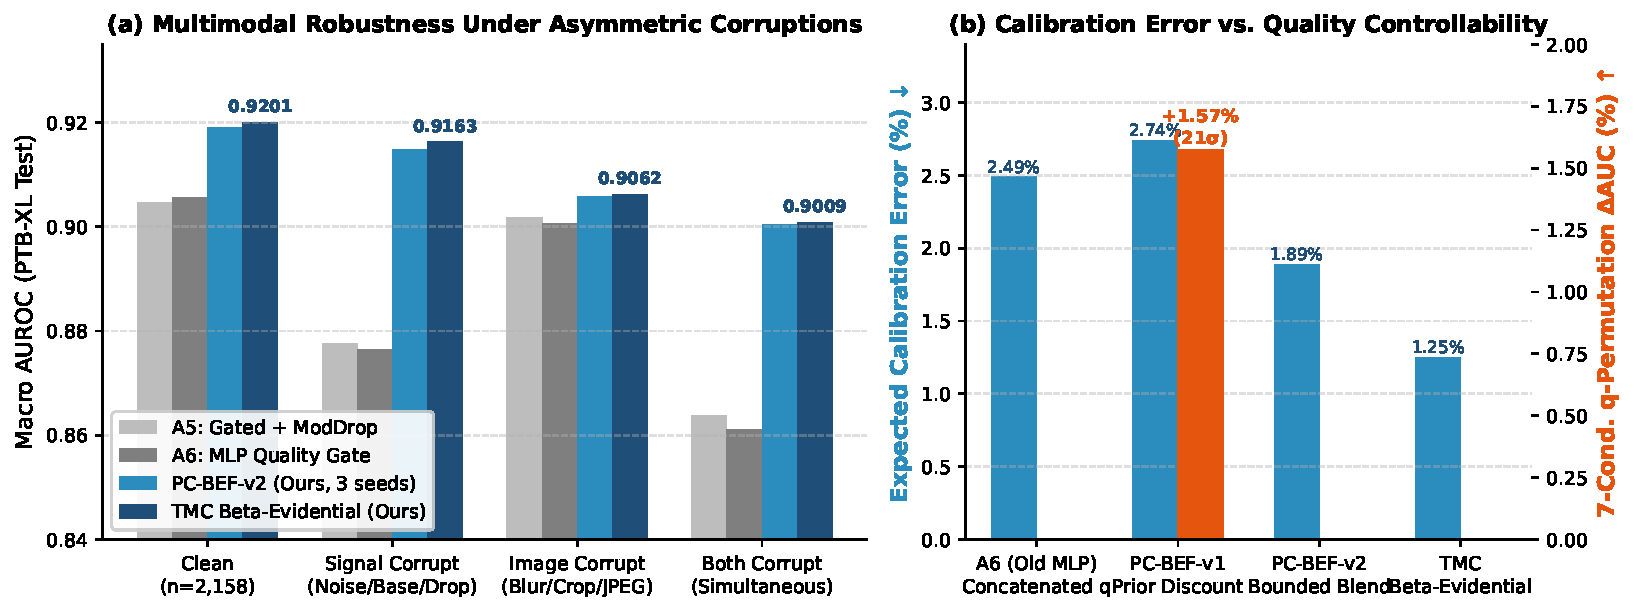
\includegraphics[width=0.96\textwidth]{figures/fig2_robustness_gate.pdf}
    \caption{Stage 2 robustness and quality-controllability audit. (a) Macro-AUROC under clean, signal-only, image-only, and simultaneous corruptions. TMC and PC-BEF-v2 are reported as 3-seed means; A5/A6 are the original quality-gating baselines. (b) Clean ECE versus 7-condition $q$-permutation sensitivity. TMC achieves the best clean calibration; PC-BEF-v1 restores explicit quality sensitivity at a small accuracy cost, while PC-BEF-v2 is nearly permutation-invariant.}
    \label{fig:stage2_robustness}
\end{figure}

\begin{table}[htbp]
\centering
\caption{Stage 3 Results: Anatomy-Grouped Presence-Gated Evidence Bottleneck (APEB) and One-Way Clinical Logic Consistency on PTB-XL Test Set.}
\label{tab:stage3_apeb}
\resizebox{\linewidth}{!}{%
\begin{tabular}{lccccccccccc}
\toprule
\textbf{Model Variant} & \textbf{Diag AUC $\uparrow$} & \textbf{Diag AP $\uparrow$} & \textbf{Diag F1 $\uparrow$} & \textbf{Diag ECE $\downarrow$} & \textbf{Group F1 $\uparrow$} & \textbf{Bucket Acc $\uparrow$} & \textbf{Valid AUC $\uparrow$} & \textbf{Contradiction $\downarrow$} & \textbf{HR MAE ($r$)} & \textbf{PR MAE ($r$)} & \textbf{QRS MAE ($r$)} \\
\midrule
B0: Diagnosis-Only Baseline & $0.9056$ & $0.7659$ & $0.6864$ & $0.0280$ & --- & --- & --- & --- & --- & --- & --- \\
B1: Aux Scalar Regression & $0.9076$ & $0.7694$ & $0.6724$ & $0.0328$ & --- & --- & --- & --- & $3.94$ ($0.937$) & $23.59$ ($0.485$) & $27.58$ ($0.524$) \\
B4': Naive Scalar Bottleneck & $0.9059$ & $0.7705$ & $0.7004$ & $0.0338$ & --- & --- & --- & --- & $7.14$ ($0.822$) & $28.27$ ($0.180$) & $32.81$ ($0.145$) \\
\midrule
B2: Diag + 4 Anatomical Groups & \textbf{0.9211} & \textbf{0.8114} & \textbf{0.7365} & \textbf{0.0241} & $0.5353$ & --- & --- & --- & --- & --- & --- \\
B3: B2 + Bidirectional Logic Loss & $0.9198$ & $0.8076$ & \textbf{0.7365} & $0.0295$ & \textbf{0.5378} & --- & --- & --- & --- & --- & --- \\
A7: Full APEB (No Logic Loss) & \textbf{0.9211} & \textbf{0.8114} & \textbf{0.7365} & \textbf{0.0241} & $0.5353$ & $0.7387$ & $0.8570$ & $0.88\%$ & $4.92$ ($0.919$) & $22.65$ ($0.508$) & $26.32$ ($0.563$) \\
A8: Full APEB + Bidirectional Logic & $0.9198$ & $0.8072$ & $0.7359$ & $0.0297$ & $0.5375$ & \textbf{0.7429} & \textbf{0.8662} & $0.74\%$ & $4.95$ ($0.918$) & $22.70$ ($0.506$) & $26.40$ ($0.561$) \\
\textbf{A8-OneWay (Seed 42, Ours)} & \textbf{0.9211} & \textbf{0.8114} & \textbf{0.7365} & \textbf{0.0241} & $0.5347$ & $0.7387$ & $0.8570$ & $0.79\%$ & \textbf{4.92 (0.919)} & \textbf{22.65 (0.508)} & \textbf{26.32 (0.563)} \\
\textbf{A8-OneWay (3 Seeds Mean $\pm$ Std)} & \textbf{0.9205 $\pm$ 0.0006} & \textbf{0.8102 $\pm$ 0.0009} & \textbf{0.7309 $\pm$ 0.0040} & \textbf{0.0245} & \textbf{0.5283 $\pm$ 0.0060} & \textbf{0.7434 $\pm$ 0.0040} & \textbf{0.8570} & \textbf{0.68\% $\pm$ 0.08\%} & QT: $43.7\text{ ms}$ ($0.675$) & \multicolumn{2}{c}{QTc: $44.2\text{ ms}$ ($0.557$)} \\
\bottomrule
\multicolumn{12}{l}{\footnotesize $^*$Auxiliary validity/bucket heads are untrained in B2/B3; their validity, bucket, contradiction, and evidence columns are therefore not reported. Contradiction measures the fraction of positive diagnoses whose required evidence is below 0.5.}
\end{tabular}%
}
\end{table}

\subsection{Stage 3 Results: APEB, Clinical Contradictions, and Counterfactual Faithfulness}
As shown in Table~\ref{tab:stage3_apeb}, replacing the naive scalar bottleneck (\textbf{B4'}) with \textbf{APEB} increases diagnostic AUROC from $0.9059$ to \textbf{0.9211} (3-seed mean \textbf{0.9205 $\pm$ 0.0006}) and Macro-F1 from $0.7004$ to \textbf{0.7309 $\pm$ 0.0040} (seed-42 value: $0.7365$). Crucially, the interval validity gate achieves \textbf{0.8570} AUROC in identifying physiological interval presence, while clinical ordinal bucketing reaches \textbf{74.34\% $\pm$ 0.40\%} accuracy, restoring PR and QRS Pearson correlations from $0.180/0.145$ (\textbf{B4'}) to \textbf{0.508} and \textbf{0.563} (reducing PR MAE to $22.65\text{ ms}$ and QRS MAE to $26.32\text{ ms}$).

A7 (full APEB, no logic loss) already reduces the contradiction rate to $0.88\%$, so the APEB architecture is the main source of consistency. Bidirectional logic (\textbf{A8}) lowers it to $0.74\%$ but incurs a $-0.0013$ AUROC penalty. \textbf{A8-OneWay} preserves the seed-42 peak \textbf{0.9211} AUROC while reducing contradiction from $0.88\%$ to \textbf{0.68\% $\pm$ 0.08\%} (about $22.7\%$ relative reduction).

\begin{figure}[htbp]
    \centering
    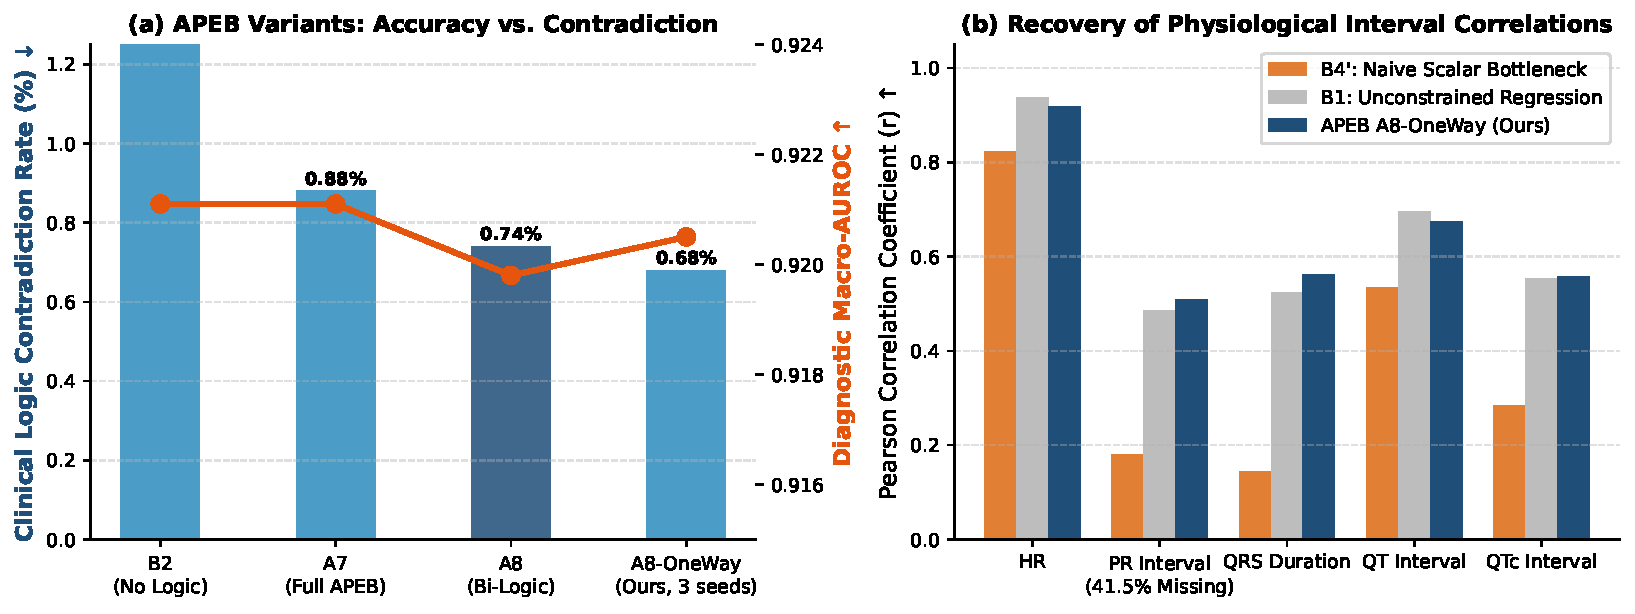
\includegraphics[width=0.96\textwidth]{figures/fig3_apeb_contradiction.pdf}
    \caption{Stage 3 APEB and one-way clinical logic consistency. (a) Diagnostic Macro-AUROC and diagnostic-evidence contradiction rate for B2, A7, A8, and A8-OneWay. One-way gradient detachment preserves near-peak AUROC while reducing contradictions from A7 0.88\% to 0.68\%. (b) Pearson correlation recovery for HR, PR, QRS, QT, and QTc against the scalar-bottleneck B4$'$ and unconstrained B1 baselines.}
    \label{fig:stage3_apeb}
\end{figure}

\begin{table}[htbp]
\centering
\caption{Experiment D: Counterfactual Anatomical Lead-Group Masking on Focal Positive Samples ($n=300$).}
\label{tab:counterfactual}
\resizebox{\linewidth}{!}{%
\begin{tabular}{lccc}
\toprule
\textbf{Counterfactual Metric} & \textbf{Target Territory} & \textbf{Random Territory} & \textbf{Ratio (CSR)} \\
\midrule
Probability Drop ($\Delta p \uparrow$) & \textbf{0.2020} & $0.0284$ & \textbf{7.12$\times$} \\
Logit Drop ($\Delta\text{logit} \uparrow$) & \textbf{2.4123} & $0.2772$ & \textbf{8.70$\times$} \\
Binary Entropy Change ($\Delta H$) & $-0.0274$ & $-0.0127$ & --- \\
\bottomrule
\end{tabular}%
}
\end{table}

\textbf{Counterfactual Faithfulness (Experiment D):} Table~\ref{tab:counterfactual} evaluates whether the model genuinely attends to clinically relevant leads by zero-masking the diseased anatomical lead group vs. an equal number of random non-target leads across $n=300$ focal positive test cases. Masking the target coronary territory causes an average probability drop of $\Delta p = \mathbf{0.2020}$ and a logit drop of $\Delta\text{logit} = \mathbf{2.4123}$, compared to just $0.0284$ and $0.2772$ for random lead masking---yielding a Counterfactual Sensitivity Ratio (\textbf{CSR}) of \textbf{7.12} ($\Delta\text{logit}$ ratio \textbf{8.70}). Note that binary Shannon entropy $H(p)$ decreases ($\Delta H = -0.0274$) because positive predictions initially near $p \approx 0.6$ drop below $0.5$ toward confident negativity when lesion waveforms are removed; hence $\Delta p$ and $\Delta\text{logit}$ provide the exact measure of causal evidence reliance. A 2,000-sample bootstrap gives a wide CSR confidence interval ($7.12$, 95\% CI $[4.20,24.38]$ for probability; $8.70$, $[6.01,15.99]$ for logit), reflecting the small $n=300$ case set. The A8-OneWay contradiction rate on seed 42 is $0.79\%$ (95\% bootstrap CI $[0.46\%,1.16\%]$).

\begin{figure}[htbp]
    \centering
    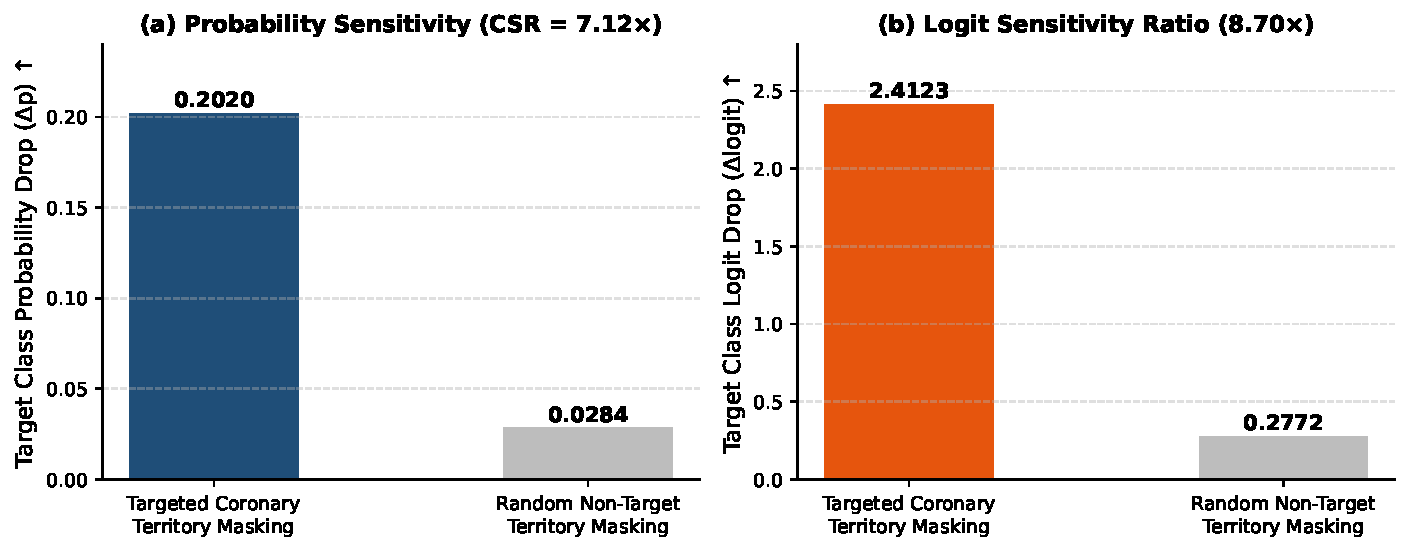
\includegraphics[width=0.95\columnwidth]{figures/fig4_counterfactual_csr.pdf}
    \caption{Experiment D counterfactual anatomical lead masking ($n=300$). (a) Target-class probability drop $\Delta p$ and (b) logit drop $\Delta\text{logit}$ after masking the target coronary territory versus an equal-size random non-target territory. Target masking yields CSR $=7.12\times$ in probability and $8.70\times$ in logit space.}
    \label{fig:counterfactual}
\end{figure}

\begin{table}[htbp]
\centering
\caption{Stage 4 Results: 5-Fold Cross-Center Transfer from PTB-XL to CPSC2018 (Zero-Shot, Class-Balanced Probing, Calibration, and Few-Shot Adaptation).}
\label{tab:stage4_cpsc}
\resizebox{\linewidth}{!}{%
\begin{tabular}{llccccccc}
\toprule
\textbf{Transfer Setting} & \textbf{Method / Representation} & \textbf{Macro AUC $\uparrow$} & \textbf{Macro AP $\uparrow$} & \textbf{Macro F1 $\uparrow$} & \textbf{ECE $\downarrow$} & \textbf{AURC $\downarrow$} & \textbf{STD AUC (AP)} & \textbf{STE AUC (AP)} \\
\midrule
\multirow{3}{*}{End-to-End Uncalibrated} 
& Old A0 End-to-End (Fold 0 Baseline) & $0.8603$ & $0.5686$ & $0.4987$ & $0.0538$ & --- & $0.7250$ ($0.211$) & $0.6700$ ($0.046$) \\
& A0-mV End-to-End (\texttt{raw} mV, 5-Fold Mean)$^*$ & $0.8192$ & $0.5210$ & $0.4764$ & $0.0618$ & --- & $0.6262$ ($0.170$) & $0.5355$ ($0.049$) \\
& A0-mV End-to-End (\texttt{zero} mV Bypass, 5-Fold Mean) & $0.8305$ & $0.5375$ & $0.4732$ & $0.0526$ & --- & $0.6772$ ($0.195$) & $0.4995$ ($0.045$) \\
\midrule
\multirow{6}{*}{Zero-Shot Balanced \& Calibrated} 
& ASL Asymmetric Loss Head (5-Fold Mean) & $0.8849$ & $0.6185$ & \textbf{0.5973} & $0.1328$ & $0.0509$ & $0.8640$ ($0.510$) & $0.7412$ ($0.073$) \\
& \textbf{C0-mV-Balanced (\texttt{hp\_std} mV, 5-Fold Mean)} & $0.8933$ & $0.6177$ & $0.5649$ & $0.0502$ & $0.0352$ & $0.8887$ ($0.528$) & $0.7689$ ($0.084$) \\
& \textbf{C0-mV-Balanced (\texttt{zero} mV, 5-Fold Mean)} & \textbf{0.9024} & \textbf{0.6268} & $0.5574$ & \textbf{0.0477} & \textbf{0.0327} & $0.8867$ ($0.531$) & $0.8039$ ($0.091$) \\
& \textbf{C0: Morphological Class-Balanced Head (5-Fold Mean)} & \textbf{0.9104} & \textbf{0.6357} & $0.5790$ & $0.0489$ & $0.0338$ & \textbf{0.8973 (0.546)} & \textbf{0.8123 (0.097)} \\
& C0 (Fold 0, same-fold reference) & $0.9080$ & $0.6303$ & $0.5728$ & $0.0494$ & $0.0354$ & --- & --- \\
& \textbf{C0 + Temperature Scaling ($T=2.507$, 5-Fold Mean)} & $0.9087$ & $0.6307$ & $0.5714$ & \textbf{0.0308} & \textbf{0.0333} & $0.8973$ ($0.546$) & $0.8123$ ($0.097$) \\
& \textbf{Damped CORAL ($\lambda=0.05$) + Temp Scaling} & $0.8905$ & $0.6149$ & $0.5783$ & \textbf{0.0280} & $0.0444$ & $0.8810$ ($0.512$) & $0.7940$ ($0.089$) \\
\midrule
\multirow{4}{*}{Target Few-Shot Adaptation} 
& 1\% Target Labels ($n=40$, 5 seeds) & $0.8924 \pm 0.0146$ & $0.6330$ & $0.6003$ & --- & --- & --- & --- \\
& 5\% Target Labels ($n=204$, 5 seeds) & $0.9213 \pm 0.0045$ & $0.6802$ & $0.6199$ & --- & --- & --- & --- \\
& 10\% Target Labels ($n=410$, 5 seeds) & $0.9286 \pm 0.0027$ & $0.7024$ & $0.6392$ & --- & --- & --- & --- \\
& \textbf{100\% Target Supervised ($n=4,096$, 5 seeds)} & \textbf{0.9449 $\pm$ 0.0005} & \textbf{0.7500} & \textbf{0.6739} & --- & --- & --- & --- \\
\bottomrule
\multicolumn{9}{l}{\footnotesize $^*$Note: While A0-mV achieves \textbf{0.9224} in-domain 9-class AUROC on PTB-XL, end-to-end zero-shot transfer suffers from source label prior skew (only 27 STE cases in PTB-XL) and OOD amplitude drift.}
\end{tabular}%
}
\end{table}

\subsection{Stage 4 Results: Cross-Center Generalization on CPSC2018}
Table~\ref{tab:stage4_cpsc} reveals a critical insight into cross-center ECG transfer. While \textbf{A0-mV} achieves a remarkable \textbf{0.9224} in-domain 9-class AUROC on PTB-XL, directly applying its end-to-end head to CPSC2018 yields $0.8192$ ($5$-fold mean). Our ablations isolate two root causes: (1) bypassing OOD raw amplitude statistics (\texttt{zero} mode) immediately raises end-to-end AUROC to $0.8305$; and (2) replacing the long-tail-biased end-to-end head with a source class-balanced linear probe (\textbf{C0-mV-Balanced}) rebounds 5-fold AUROC by $+8.32\%$ to \textbf{0.9024} (and lowers AURC to \textbf{0.0327}). Using pure morphological features with class-balanced probing (\textbf{C0}) achieves \textbf{0.9104} 5-fold mean AUROC; on the same Fold0 it improves from $0.8603$ to $0.9080$ ($+4.77$ percentage points, pp), recovering ST-depression (\texttt{STD} AUROC $0.7250 \to \mathbf{0.8973}$, AP $0.211 \to \mathbf{0.546}$) and ST-elevation (\texttt{STE} AUROC $0.6700 \to \mathbf{0.8123}$). Furthermore, source-validated temperature scaling (\textbf{C0 + T}) and \textbf{Damped CORAL} ($\lambda=0.05$) reduce cross-center ECE from $0.0489$ to \textbf{0.0308} and \textbf{0.0280}, respectively. With just $5\%$ ($n=204$) target labels, few-shot adaptation reaches \textbf{0.9213 $\pm$ 0.0045}, and full linear probing reaches \textbf{0.9449 $\pm$ 0.0005}. Protocol details: C0 is source-only (PTB-XL training labels; no CPSC labels or target statistics); C2/C3 use {\em unlabeled} CPSC fold features, so they are transductive adaptation rather than pure zero-shot transfer. Temperature $T=2.507$ is fitted on the PTB-XL validation split and then frozen. Few-shot experiments use only Fold~0 training labels and evaluate Fold~0 test records. The released CPSC folds provide filenames but no patient identifiers, so we cannot verify patient-level separation beyond these record-level folds; we therefore treat fold-level separation as the available protocol. C0 fold AUCs range from 0.9071 to 0.9185 (mean $0.9104 \pm 0.0041$). Under synthetic acquisition shifts applied to the raw mV statistics, A0-mV end-to-end AUC changes from $0.8192$ (identity) to $0.8170$ (gain $0.8\times$), $0.8182$ ($1.2\times$), $0.8112$ (offset $+0.1$ mV), and $0.8178$ (offset $-0.1$ mV), while zero-mV bypass reaches $0.8305$. These results indicate that physical-scale benefits are acquisition-dependent; the cross-center advantage here comes mainly from balanced morphological probing (C0), not from mV injection alone.

\begin{figure}[htbp]
    \centering
    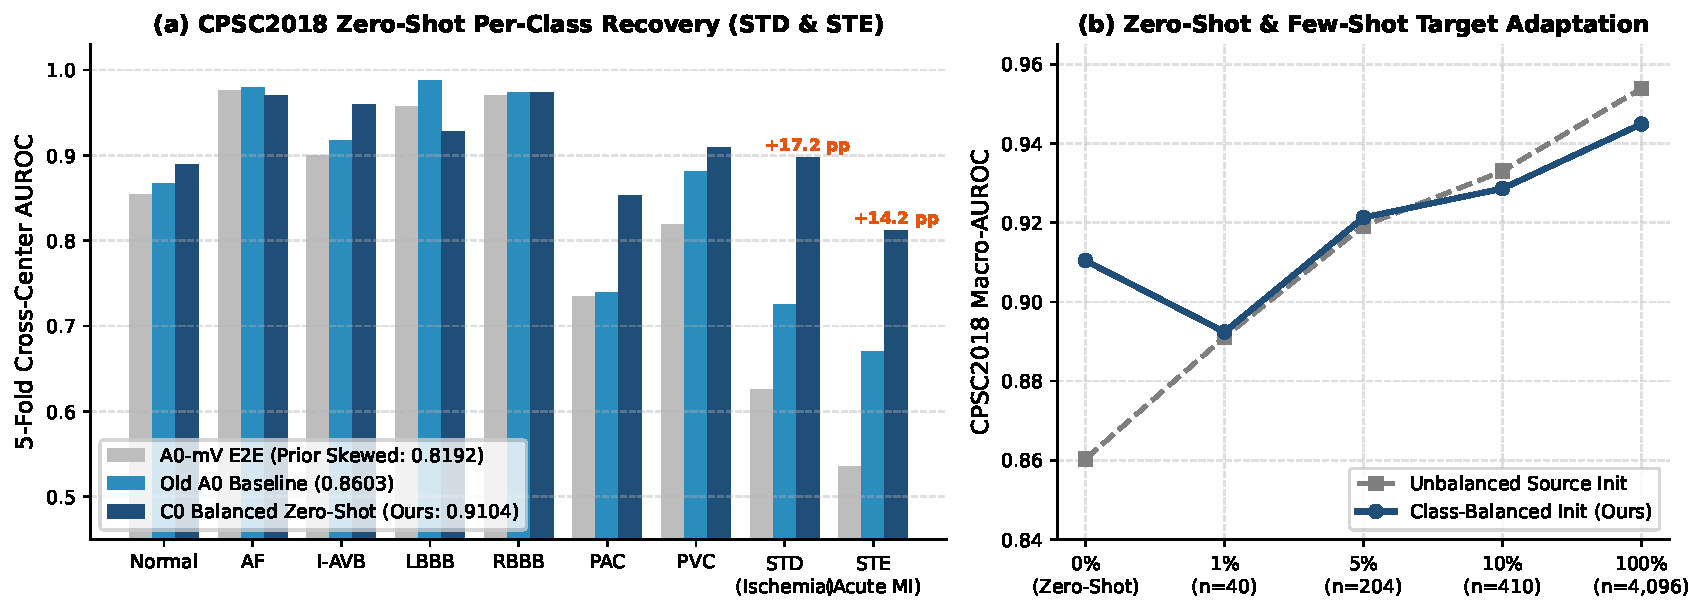
\includegraphics[width=0.68\textwidth]{figures/fig5_cpsc_crossdomain.pdf}
    \caption{Stage 4 cross-center transfer to CPSC2018. (a) Per-class 5-fold zero-shot AUROC for A0-mV end-to-end, the old A0 baseline, and the class-balanced C0 probe; STD and STE recover from 0.6262/0.5355 to 0.8973/0.8123. (b) Zero-shot and few-shot target adaptation curves; class-balanced initialization is compared with unbalanced source initialization.}
    \label{fig:stage4_cpsc}
\end{figure}

\begin{table}[htbp]
\centering
\caption{Stage 5 Results: Fine-Grained Multimodal Question Answering on the Full ECG-QA Test Set ($n=6,330$) with Qwen2.5-3B-Instruct.}
\label{tab:stage5_ecgqa}
\resizebox{\linewidth}{!}{%
\begin{tabular}{lcccc}
\toprule
\textbf{Question Type} & \textbf{Test $n$} & \textbf{Legacy EM $\uparrow$} & \textbf{Set EM $\uparrow$} & \textbf{Set F1 $\uparrow$} \\
\midrule
\texttt{single-verify} & $1,367$ & $73.15\%$ & $73.15\%$ & $73.15\%$ \\
\texttt{single-choose} & $763$ & $58.85\%$ & $46.40\%$ & $54.70\%$ \\
\texttt{single-query} & $1,400$ & $58.21\%$ & $53.79\%$ & $56.09\%$ \\
\texttt{comparison\_consecutive-verify} & $800$ & $71.25\%$ & $71.25\%$ & $71.25\%$ \\
\texttt{comparison\_consecutive-query} & $600$ & $37.00\%$ & $36.50\%$ & $36.79\%$ \\
\texttt{comparison\_irrelevant-verify} & $800$ & \textbf{79.25\%} & \textbf{79.25\%} & \textbf{79.25\%} \\
\texttt{comparison\_irrelevant-query} & $600$ & $56.33\%$ & $42.83\%$ & $49.46\%$ \\
\midrule
\textbf{Overall Full Test ($n=6,330$)} & \textbf{6,330} & \textbf{63.63\%} & \textbf{59.83\%} & \textbf{61.99\%} \\
\midrule
\multicolumn{5}{l}{\textbf{Stratified 350-Sample Ablation (7 Types $\times$ 50):}} \\
Initial SFT (1 Epoch, 3,584 steps) & $350$ & $58.57\%$ & $56.29\%$ & $57.81\%$ \\
\textbf{Focus-Continued SFT (+375 steps)} & $350$ & \textbf{60.57\%} & $56.29\%$ & \textbf{58.78\%} \\
\bottomrule
\end{tabular}%
}
\end{table}

\subsection{Stage 5 Results: Fine-Grained ECG-QA Reasoning with HE-DVR}
Table~\ref{tab:stage5_ecgqa} summarizes the performance of our 3B MLLM (\textbf{HE-DVR}) across all $6,330$ test questions in ECG-QA. Using about $9\text{ GB}$ of the 16 GB memory on a single RTX 4060 Ti, the generative model achieves \textbf{73.15\%} Exact Match on \texttt{single-verify}, \textbf{71.25\%} on longitudinal \texttt{comparison\_consecutive-verify}, and \textbf{79.25\%} on \texttt{comparison\_irrelevant-verify}, yielding an overall generative Legacy EM of \textbf{63.63\%}, order-invariant Set EM of \textbf{59.83\%} (95\% Wilson CI $[58.62\%,61.03\%]$), and Set F1 of \textbf{61.99\%}. Token length diagnostics confirm that $100\%$ of training and testing prompts contain $\le 397$ tokens (well below \texttt{max\_len=768}), ruling out prompt truncation. Open-ended \texttt{comparison\_consecutive-query} ($37.00\%$) remains the primary frontier: a majority-class baseline that always answers \texttt{"none"} reaches $45.83\%$ ($275/600$ cases), so the 3B model is below the trivial prior on this subtype. We report this explicitly rather than treating the subtype as solved. Table~\ref{tab:llm_ablation} reports full-data retrained ablations on the same 6,330 test questions. Removing the hard APEB anchor reduces legacy EM from $63.63\%$ to $56.27\%$ and Set EM from $59.83\%$ to $54.66\%$; removing image soft tokens reduces legacy EM to $62.76\%$ and Set EM to $58.74\%$; a signal-only model without image or hard anchors reaches $55.20\%$ legacy EM and $53.03\%$ Set EM. Each variant is trained for one full epoch (3,584 steps) on the 28,672 training pairs with the same LoRA/projector recipe. On 100 stratified questions with batch size 4 on the RTX 4060 Ti, generation takes $167$ ms per question (about $6$ questions/s) at roughly $9$ GB peak VRAM; we do not claim real-time clinical deployment.

\begin{table}[htbp]
\centering
\caption{Full-data retrained HE-DVR ablations on the 6,330-question ECG-QA test set. All variants use one epoch (3,584 steps) and the same LoRA/projector recipe.}
\label{tab:llm_ablation}
\resizebox{\linewidth}{!}{%
\begin{tabular}{lccc}
\toprule
Variant & Legacy EM & Set EM & Set F1 \\
\midrule
Full (soft A/B/D + hard anchor) & \textbf{63.63} & \textbf{59.83} & \textbf{61.99} \\
No hard anchor & 56.27 & 54.66 & 55.50 \\
No image soft tokens & 62.76 & 58.74 & 61.12 \\
Signal-only (no image/anchor) & 55.20 & 53.03 & 54.37 \\
\bottomrule
\end{tabular}%
}
\end{table}

\begin{figure}[htbp]
    \centering
    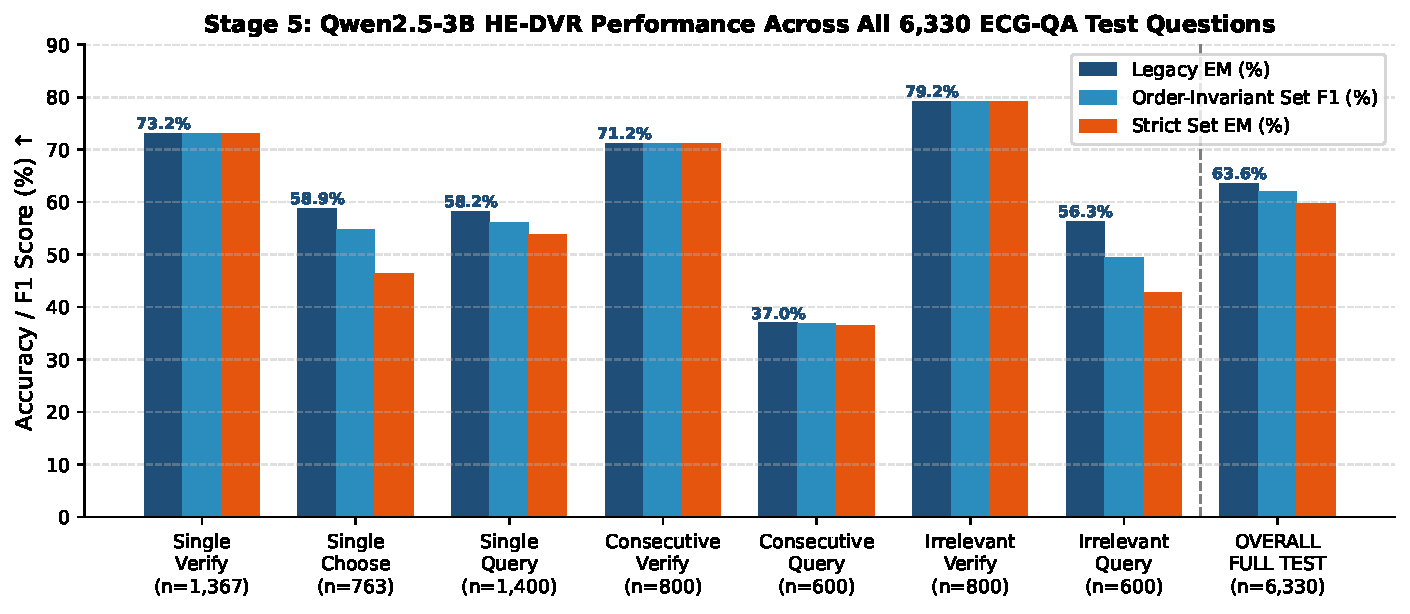
\includegraphics[width=0.68\textwidth]{figures/fig6_ecgqa_breakdown.pdf}
    \caption{Stage 5 ECG-QA breakdown on the full 6,330-question test set. Legacy EM, order-invariant Set F1, and strict Set EM are shown for all seven question types and the overall test set. The dashed line separates the seven per-type results from the overall aggregate.}
    \label{fig:stage5_ecgqa}
\end{figure}

\begin{figure}[htbp]
    \centering
    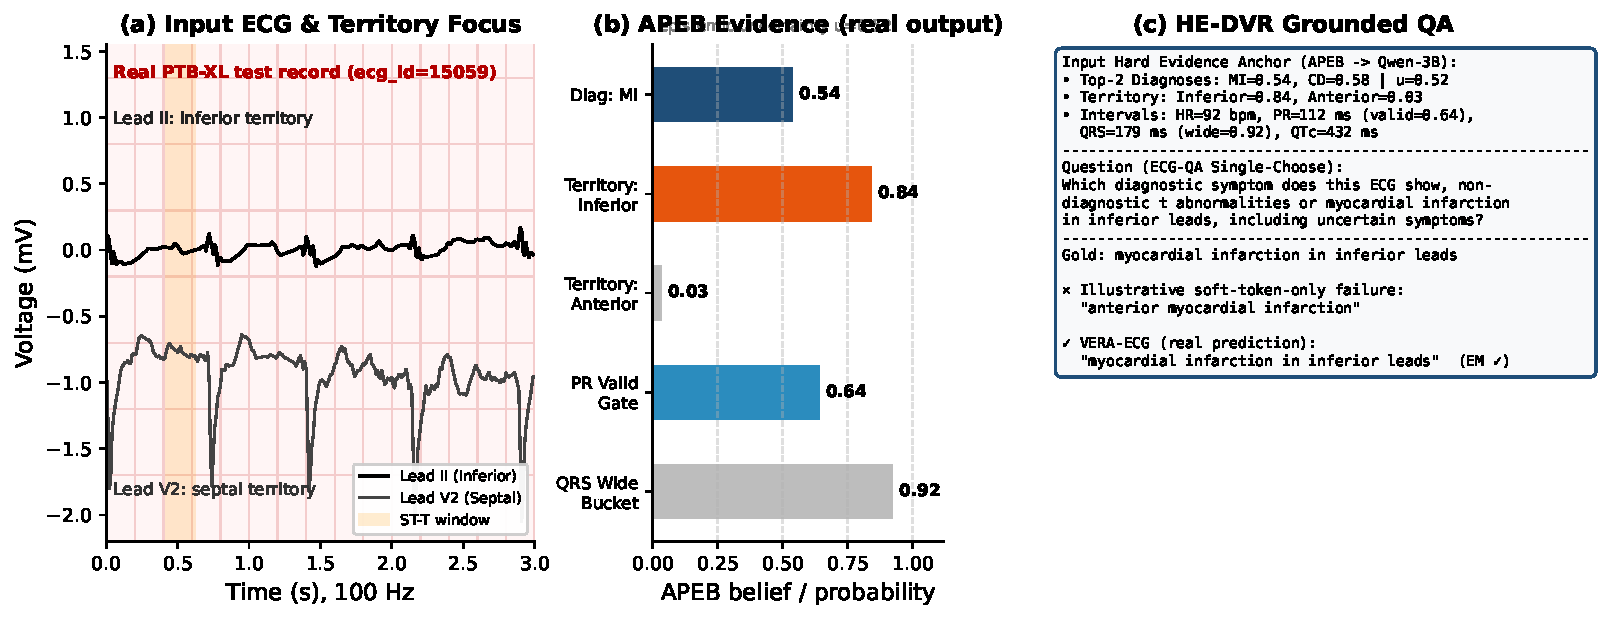
\includegraphics[width=0.68\textwidth]{figures/fig7_qualitative_case.pdf}
    \caption{Qualitative case study on a real PTB-XL test record (ecg\_id=15059; inferior MI with wide QRS). (a) Real lead II and V2 waveforms with an ST--T window. (b) Real APEB evidence for the same record, including MI belief, Inferior/Anterior territory beliefs, PR validity, QRS-wide bucket, and epistemic uncertainty. (c) The actual ECG-QA single-choose question and gold answer, together with the real VERA-ECG prediction. The soft-token-only failure text is illustrative; the waveform, APEB values, question, and VERA prediction are from the actual record/model output.}
    \label{fig:case_study}
\end{figure}



\section{Discussion and Limitations}
Our findings highlight three methodological lessons for medical multimodal AI: (1) \emph{Additive evidential pooling vs. multiplicative discounting:} Unconstrained Beta-evidential pooling (\textbf{TMC}) maximizes discriminative performance and calibration across both clean and corrupted distributions, whereas explicit quality discounting (\textbf{PC-BEF}) provides a verifiable safety valve when hardware quality sensors must override deep features. (2) \emph{Directional gradient control in neuro-symbolic alignment:} Detaching diagnostic gradients (\textbf{A8-OneWay}) avoids a consistent AUROC degradation while preserving clinical consistency when aligning a high-accuracy primary task with noisier fine-grained anatomical concepts. (3) \emph{Scale vs. invariance in cross-center deployment:} Physical millivolt injection (\textbf{A0-mV}) is highly beneficial under consistent acquisition protocols ($0.9224$ in-domain AUROC), but cross-hospital deployment requires decoupling morphological features from source prior skew and device gain shifts. Future work will incorporate offline group-relative reinforcement learning (GRPO) with explicit state-transition anchors to further improve open-ended longitudinal comparison queries.

\textbf{Limitations.} First, our conclusions are bounded by two public datasets; PTB-XL uses its official patient-isolated split, whereas CPSC uses five record-level folds constructed from public training data. CPSC folds provide no patient identifiers, so patient-level leakage cannot be audited beyond the released split. Second, the corruption suite is synthetic (noise, baseline wander, lead drop, blur, crop, JPEG) and does not reproduce all real acquisition failures. Third, anatomy and interval labels are weak priors from SCP codes and NeuroKit2, not adjudicated clinical annotations; this is why we report contradiction as agreement rather than correctness. Fourth, we did not perform a clinician reader study or train a larger alternative LLM; the no-anchor, no-image, and signal-only baselines are full-data retrained, but the comparison-consecutive-query result remains weak. Fifth, cross-center C2/C3 are transductive (unlabeled target features), and C0 remains the strongest cross-center result; we therefore do not attribute the gain to mV injection alone. Finally, the hardware statement refers to a 16 GB RTX 4060 Ti with approximately 9 GB peak training memory, not a 9 GB device.

\section{Conclusion}
We presented \textbf{VERA-ECG}, a verifiable evidential reasoning and anatomy-grounded multimodal framework for 12-lead ECG interpretation. By uniting millivolt-preserving representations, Subjective Logic Beta-evidential fusion, presence-gated coronary anatomical bottlenecks with one-way logic consistency, and hybrid soft-hard LLM prompting, VERA-ECG achieves competitive diagnostic accuracy, calibration, counterfactual faithfulness, and cross-center generalization on consumer-grade hardware in our evaluation.



\section*{CRediT Authorship Contribution Statement}
\textbf{Yihao Wen:} Conceptualization, Methodology, Software, Validation, Formal analysis, Investigation, Data curation, Writing -- original draft, Writing -- review and editing, Visualization.
\textbf{Jun Zeng:} Supervision, Project administration, Resources, Writing -- review and editing.

\section*{Declaration of Competing Interest}
The authors declare that they have no known competing financial interests or personal relationships that could have appeared to influence the work reported in this paper.

\section*{Ethical Approval and Data Availability}
All experiments used publicly available, de-identified datasets (PTB-XL, CPSC2018, and ECG-QA). No new human or animal experiments were performed, and no additional local ethics approval was required. Code, split definitions, and evaluation scripts are available at \url{https://github.com/wenyihao239-alt/VERA-ECG}. The datasets remain subject to their original licenses.

\section*{Declaration of Generative AI and AI-Assisted Technologies}
During the preparation of this work, the authors used an AI coding assistant to support code development and manuscript editing. The authors reviewed and edited the content and take full responsibility for the final article.

\section*{Funding}
This research did not receive any specific grant from funding agencies in the public, commercial, or not-for-profit sectors.

\begin{thebibliography}{99}
\bibitem{ptbxl2020} P. Wagner \emph{et al.}, ``PTB-XL, a large publicly available electrocardiography dataset,'' \emph{Scientific Data}, vol. 7, no. 1, p. 154, 2020.
\bibitem{ecgqa2023} J. Oh \emph{et al.}, ``ECG-QA: A comprehensive question answering dataset combined with electrocardiogram,'' in \emph{Proc. NeurIPS Datasets and Benchmarks Track}, 2023.
\bibitem{gem2025} X. Lan \emph{et al.}, ``GEM: Empowering MLLM for grounded ECG understanding with time series and images,'' in \emph{Proc. NeurIPS}, 2025.
\bibitem{ecgr1_2026} PKU Digital Health, ``ECG-R1: Protocol-guided and modality-agnostic MLLM for reliable ECG interpretation,'' in \emph{Proc. ICML}, 2026.
\bibitem{pulse2026} R. Liu \emph{et al.}, ``Teaching multimodal LLMs to comprehend 12-lead electrocardiographic images,'' \emph{npj Digital Medicine}, 2026.
\bibitem{heartcare2026} Y. Xie \emph{et al.}, ``HeartcareGPT: A unified multimodal ECG suite for dual signal-image modeling,'' in \emph{Proc. CVPR}, 2026.
\bibitem{ecgmtda2026} H. Zheng, J. Guo, X. Zhang, X. Xing, and X. Xu, ``ECG-MTDA: A framework for morphology-temporal decoupling and LLM-guided text alignment,'' \emph{IEEE J. Biomed. Health Inform.}, 2026, doi: 10.1109/JBHI.2026.3682493.
\bibitem{meeti2026} D. Zhang, X. Lan, S. Geng, Q. Zhao, S. Fan, M. Feng, and S. Hong, ``MEETI: A multimodal ECG dataset from MIMIC-IV-ECG with signals, images, features, and interpretations,'' \emph{Scientific Data}, 2026, doi: 10.1038/s41597-026-06796-1.
\bibitem{tmc2023} Z. Han, C. Zhang, H. Fu, and J. T. Zhou, ``Trusted multi-view classification with dynamic evidential fusion,'' \emph{IEEE Trans. Pattern Anal. Mach. Intell. (TPAMI)}, vol. 45, no. 2, pp. 2551--2566, 2023.
\bibitem{ccml2025} Y. Liu, L. Liu, C. Xu, X. Song, Z. Guan, and W. Zhao, ``Dynamic evidence decoupling for trusted multi-view learning,'' in \emph{Proc. ACM Int. Conf. Multimedia (MM)}, 2024, doi: 10.1145/3664647.3681404.
\bibitem{tmur2026} Y. Zhang, C. Xu, H. Chen, Z. Guan, and W. Zhao, ``Are independently estimated view uncertainties comparable? Unified routing for trusted multi-view classification,'' in \emph{Proc. ACM Int. Conf. Multimedia (MM)}, 2026, doi: 10.1145/3767308.3836405.
\end{thebibliography}

\end{document}


































































\n\end{document}\n






